% !TeX root = ../skript.tex
% !TeX spellcheck = de_DE

\section{Visualisierung}
Das oben erwähnte Gleichungssystem haben wir im Javascript-Code verwendet, um die Resultate des Lorenzsystems auszurechnen. Der folgende Code ist das Lorenz-Modell aus dem Javascript-Code der Visualisierung. Nachfolgend ist eine Aufstellung aller Variablen im Code und in den Formeln oberhalb.

	% TODO: Beschreibung warum Durchlauf Unterschied macht, da Rückkopplungen unaufgelöst, und welche Probleme es nicht löst.
	\begin{lstlisting}[style=C]
	x = arr[i].x + ((sigma * y) - (sigma * x)) * delta;
	y = arr[i].y + ((-x * z) + (rho * x) - y) * delta;
	z = arr[i].z + ((x * y) - (beta * z)) * delta;
	\end{lstlisting}

\begin{align*}
{\renewcommand{\arraystretch}{1.2}
	\begin{tabular}{| c | c | c | c |}
		\hline
		\textbf{Bedeutung} & \textbf{Mathematisches Symbol} & \textbf{Variable im Code} & \textbf{Anfangswert}\\\hline
		Zeitschritt & $ \Delta $ & \texttt{delta} & 0.1 \\\hline
		Rayleigh Zahl & $ \sigma $ & \texttt{sigma} & 10 \\\hline
		Prandtl Zahl & $\varrho $ & \texttt{rho} & 28 \\\hline
		Wärmeausdehnung & $\beta $ & \texttt{beta}  & $ \frac{8}{3} $ \\\hline
	\end{tabular}
}
\end{align*}

Die $ x, y $ Variablen in der 1. Gleichung ist noch mit dem Wert des vorherigen Durchgangs besetzt und deshalb eine Annäherung um den echten Wert. Das gleiche gilt für alle Werte, die vor der Ausführung noch nicht gesetzt sind. 
Beim ersten Durchgang wird 0.1 als Startwert angenommen um zu verhindern, dass das Gleichungssystem gelöst ist durch den Initialwert einer Javascript Variable. 

Wenn $ \vec{0} $ eingesetzt wird löst sich das Gleichungssystem auf $ \vec{0} $. Da das Ergebnis wieder eingesetzt wird in der nächsten Runde, wird das Gleichungssystem über alle Runden $ \vec{0} $ ausgeben. Um dieses Verhalten zu verhindern lassen wir den Algorithmus etwas neben $ \vec{0} $ starten bei $ \vec{0.1} $.

Die Werte des Lorenz-Modells werden in einem Array als 3D-Vektoren abgespeichert. Diese Ortsvektoren stellen die Position der Punkte im drei dimensionalen Raum dar. Die Darstellungsobjekte an diesen Positionen besitzen die Form von \textit{Spheren}. Ein solches Objekt stellt einen Wert der Lorenzgleichungen dar und es werden 2500 Werte berechnet und dargestellt.

Die Darstellung wird mittels \textit{WebGL}\cite{WebGL} im Browser gerendert. \textit{WebGL} ist eine komplexe Software und trifft wenige Annahmen selber. Aus diesem Grund haben wir auf dieser Technologie aufbauende Middleware \textit{WhitestormJS}\cite{whitestormJS} verwendet um gute Standardeinstellungen zu bekommen.

Für die Interaktiviät der Webpage mit Animationen bei den Seitenwechsel, Textboxen und Vereinfachung des Codes ist die neue JavaScript Bibliothek \textit{VueJS}\cite{VueJS} zum Einsatz gekommen.

Dank diesen Helfern konnten wir innerhalb von etwa 30h Arbeit eine Vollständige Simulationsumgebung für das Lorenz-Modell 68 mit folgenden Charakteristiken programmieren:

\begin{itemize}
	\item 3D-Visualisierung
	\item Drehen und Zoomen
	\item Sofortiges update von 3D Visualisierung bei Paramteränderung
	\item fixe 3D-Bilder, deren Parameter konstant waren
	\item Erklärungstext
\end{itemize}

\begin{figure}
	\centering	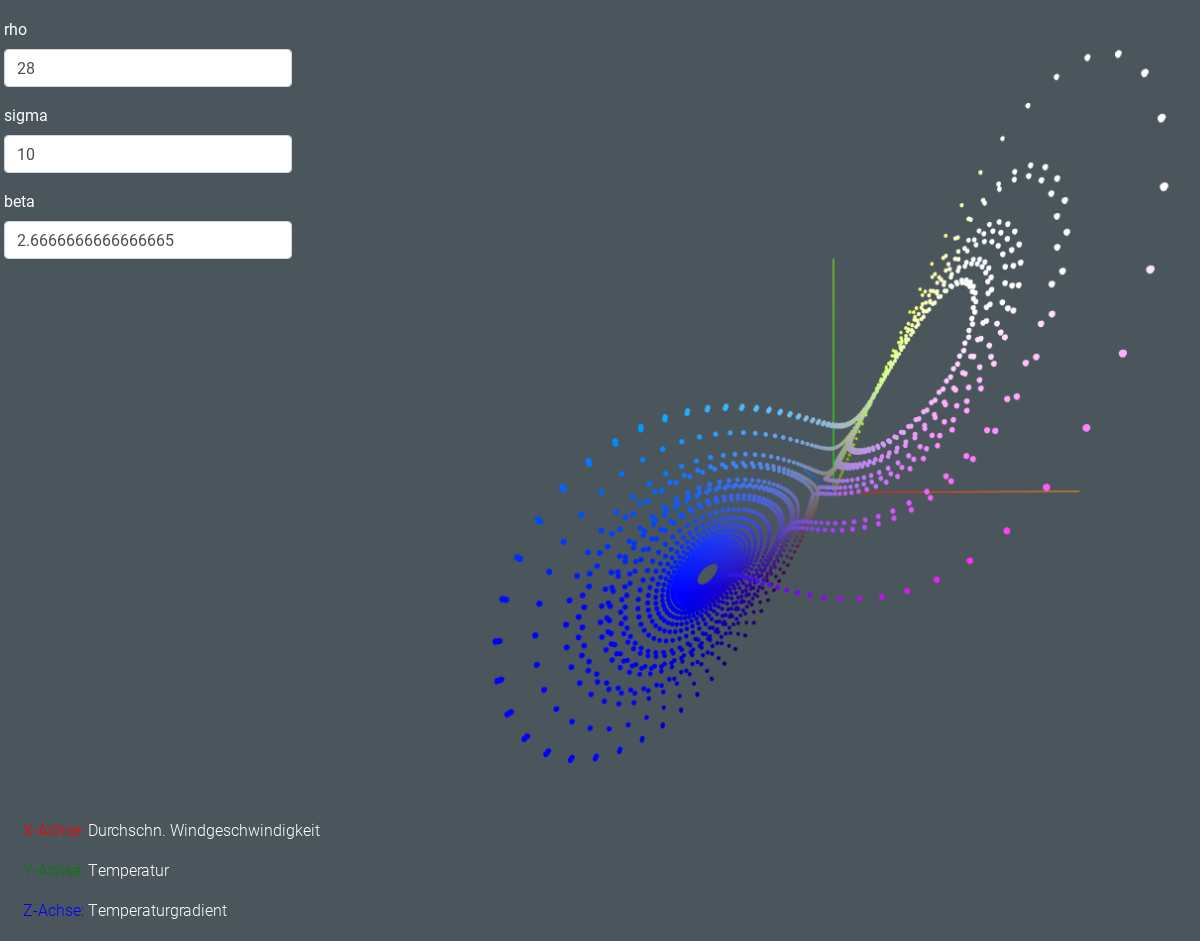
\includegraphics[height=5cm]{lorenz/assets/implementation/Visualisierung}
	\caption{Visualisierung Lorenz-Attraktor}
	\label{fig:visualisierung}
\end{figure}
